%\section{Mô phỏng thuật toán giải mã Viterbi bằng System Verilog}
\section{MÔ PHỎNG THUẬT TOÁN GIẢI MÃ VITERBI BẰNG SYSTEM VERILOG}

\subsection{Branch Metric Unit (BMU)}

\subsubsection{Block Diagram for BMU}

\begin{figure}[H]
	\centering
	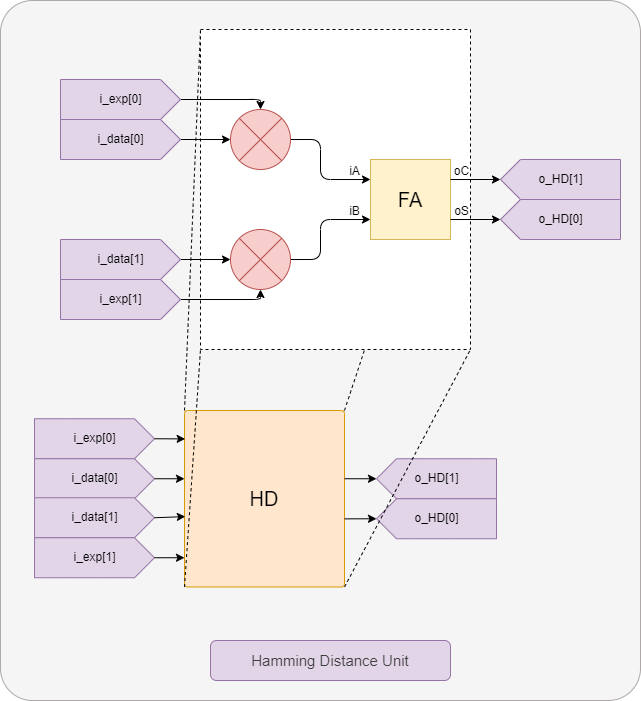
\includegraphics[width=.8\linewidth]{sections/pic/mophongbangSystemVerilog/HD_unit.png}
	\caption{Bộ tính toán khoảng cách Hamming.}
\end{figure}

\begin{figure}[H]
	\centering
	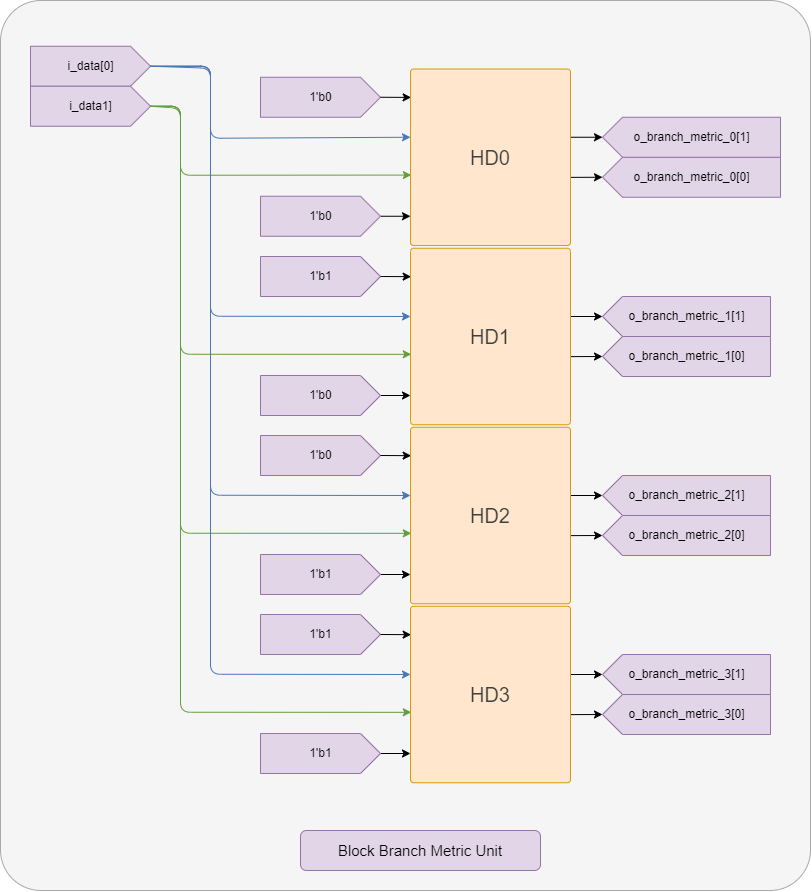
\includegraphics[width=.8\linewidth]{sections/pic/mophongbangSystemVerilog/BM_unit.png}
	\caption{Bộ BMU.}
\end{figure}

\subsubsection{IO for BMU}

\begin{table}[H]
	\centering
	\begin{tabular}{|>{\centering\arraybackslash}p{3cm}|>{\centering\arraybackslash}p{1cm}|>{\raggedright\arraybackslash}p{9cm}|}
		\hline
		\textbf{Port} & \textbf{Size} & \textbf{Function} \\
		\hline
		i\_data & 2 & Data ngõ vào bộ VD.\\
		\hline
		o\_BM\_0 & 2 & Giá trị Branch Metric sau khi tính toán với expected là 0x00\\
		\hline
		o\_BM\_1 & 2 & Giá trị Branch Metric sau khi tính toán với expected là 0x01\\
		\hline
		o\_BM\_2 & 2 & Giá trị Branch Metric sau khi tính toán với expected là 0x10\\
		\hline
		o\_BM\_3 & 2 & Giá trị Branch Metric sau khi tính toán với expected là 0x11\\
		\hline
	\end{tabular}
	\caption{Bảng sơ đồ chân của bộ BMU.}
\end{table}

\subsubsection{Chức năng của BMU}

Bộ BMU có chức tính toán Khoảng cách Hamming giữa giá trị đã ngõ vào (i\_data) và các giá trị expected. Với bộ VD $(3, 1, 2)$ thì expected word sẽ là 0x00, 0x01, 0x10, 0x11.

\begin{table}[H]
	\centering
	\begin{tabular}{|>{\centering\arraybackslash}p{3cm}|>{\centering\arraybackslash}p{3cm}|>{\centering\arraybackslash}p{3cm}|>{\centering\arraybackslash}p{3cm}|>{\centering\arraybackslash}p{3cm}|}
		\hline
		\textbf{i\_data} & \textbf{o\_BM\_0} & \textbf{o\_BM\_1} & \textbf{o\_BM\_2} & \textbf{o\_BM\_3} \\
		\hline
		00 & 00 & 01 & 01 & 10 \\
		\hline
		01 & 01 & 00 & 10 & 01 \\
		\hline
		10 & 00 & 10 & 00 & 01 \\
		\hline
		11 & 10 & 01 & 01 & 00 \\
		\hline
	\end{tabular}
	\caption{Bẳng sự thật của bộ BMU.}
\end{table}

%\begin{lstlisting}[style=StyleResult, language=Result]
%	Time: 0 | i_rst_n = 0 | i_data: 00 | o_BM_0: 00 | o_BM_1: 00 | o_BM_2: 00 | o_BM_3: 00 | o_valid: 0
%	Time: 5000 | i_rst_n = 0 | i_data: 00 | o_BM_0: 00 | o_BM_1: 00 | o_BM_2: 00 | o_BM_3: 00 | o_valid: 0
%	Time: 5000 | i_rst_n = 0 | i_data: 00 | o_BM_0: 00 | o_BM_1: 00 | o_BM_2: 00 | o_BM_3: 00 | o_valid: 0
%	Time: 5000 | i_rst_n = 0 | i_data: 00 | o_BM_0: 00 | o_BM_1: 00 | o_BM_2: 00 | o_BM_3: 00 | o_valid: 0
%	Time: 10000 | i_rst_n = 1 | i_data: 00 | o_BM_0: 00 | o_BM_1: 00 | o_BM_2: 00 | o_BM_3: 00 | o_valid: 0
%	Time: 10000 | i_rst_n = 1 | i_data: 00 | o_BM_0: 00 | o_BM_1: 00 | o_BM_2: 00 | o_BM_3: 00 | o_valid: 0
%	Time: 15000 | i_rst_n = 1 | i_data: 00 | o_BM_0: 00 | o_BM_1: 00 | o_BM_2: 00 | o_BM_3: 00 | o_valid: 0
%	Time: 15000 | i_rst_n = 1 | i_data: 00 | o_BM_0: 00 | o_BM_1: 00 | o_BM_2: 00 | o_BM_3: 00 | o_valid: 0
%	Time: 15000 | i_rst_n = 1 | i_data: 00 | o_BM_0: 00 | o_BM_1: 01 | o_BM_2: 01 | o_BM_3: 10 | o_valid: 1
%	Time: 20000 | i_rst_n = 1 | i_data: 00 | o_BM_0: 00 | o_BM_1: 01 | o_BM_2: 01 | o_BM_3: 10 | o_valid: 1
%	Time: 20000 | i_rst_n = 1 | i_data: 00 | o_BM_0: 00 | o_BM_1: 01 | o_BM_2: 01 | o_BM_3: 10 | o_valid: 1
%	Time: 25000 | i_rst_n = 1 | i_data: 00 | o_BM_0: 00 | o_BM_1: 01 | o_BM_2: 01 | o_BM_3: 10 | o_valid: 1
%	Time: 25000 | i_rst_n = 1 | i_data: 00 | o_BM_0: 00 | o_BM_1: 01 | o_BM_2: 01 | o_BM_3: 10 | o_valid: 1
%	Time: 25000 | i_rst_n = 1 | i_data: 00 | o_BM_0: 00 | o_BM_1: 01 | o_BM_2: 01 | o_BM_3: 10 | o_valid: 1
%	Time: 30000 | i_rst_n = 1 | i_data: 00 | o_BM_0: 00 | o_BM_1: 01 | o_BM_2: 01 | o_BM_3: 10 | o_valid: 1
%	Time: 30000 | i_rst_n = 1 | i_data: 00 | o_BM_0: 00 | o_BM_1: 01 | o_BM_2: 01 | o_BM_3: 10 | o_valid: 1
%	Time: 35000 | i_rst_n = 1 | i_data: 00 | o_BM_0: 00 | o_BM_1: 01 | o_BM_2: 01 | o_BM_3: 10 | o_valid: 1
%	Time: 35000 | i_rst_n = 1 | i_data: 01 | o_BM_0: 00 | o_BM_1: 01 | o_BM_2: 01 | o_BM_3: 10 | o_valid: 1
%	Time: 35000 | i_rst_n = 1 | i_data: 01 | o_BM_0: 01 | o_BM_1: 00 | o_BM_2: 10 | o_BM_3: 01 | o_valid: 1
%	Time: 40000 | i_rst_n = 1 | i_data: 01 | o_BM_0: 01 | o_BM_1: 00 | o_BM_2: 10 | o_BM_3: 01 | o_valid: 1
%	Time: 40000 | i_rst_n = 1 | i_data: 01 | o_BM_0: 01 | o_BM_1: 00 | o_BM_2: 10 | o_BM_3: 01 | o_valid: 1
%	Time: 45000 | i_rst_n = 1 | i_data: 01 | o_BM_0: 01 | o_BM_1: 00 | o_BM_2: 10 | o_BM_3: 01 | o_valid: 1
%	Time: 45000 | i_rst_n = 1 | i_data: 01 | o_BM_0: 01 | o_BM_1: 00 | o_BM_2: 10 | o_BM_3: 01 | o_valid: 1
%	Time: 45000 | i_rst_n = 1 | i_data: 01 | o_BM_0: 01 | o_BM_1: 00 | o_BM_2: 10 | o_BM_3: 01 | o_valid: 1
%	Time: 50000 | i_rst_n = 1 | i_data: 01 | o_BM_0: 01 | o_BM_1: 00 | o_BM_2: 10 | o_BM_3: 01 | o_valid: 1
%	Time: 50000 | i_rst_n = 1 | i_data: 01 | o_BM_0: 01 | o_BM_1: 00 | o_BM_2: 10 | o_BM_3: 01 | o_valid: 1
%	Time: 55000 | i_rst_n = 1 | i_data: 01 | o_BM_0: 01 | o_BM_1: 00 | o_BM_2: 10 | o_BM_3: 01 | o_valid: 1
%	Time: 55000 | i_rst_n = 1 | i_data: 10 | o_BM_0: 01 | o_BM_1: 00 | o_BM_2: 10 | o_BM_3: 01 | o_valid: 1
%	Time: 55000 | i_rst_n = 1 | i_data: 10 | o_BM_0: 01 | o_BM_1: 10 | o_BM_2: 00 | o_BM_3: 01 | o_valid: 1
%	Time: 60000 | i_rst_n = 1 | i_data: 10 | o_BM_0: 01 | o_BM_1: 10 | o_BM_2: 00 | o_BM_3: 01 | o_valid: 1
%	Time: 60000 | i_rst_n = 1 | i_data: 10 | o_BM_0: 01 | o_BM_1: 10 | o_BM_2: 00 | o_BM_3: 01 | o_valid: 1
%	Time: 65000 | i_rst_n = 1 | i_data: 10 | o_BM_0: 01 | o_BM_1: 10 | o_BM_2: 00 | o_BM_3: 01 | o_valid: 1
%	Time: 65000 | i_rst_n = 1 | i_data: 10 | o_BM_0: 01 | o_BM_1: 10 | o_BM_2: 00 | o_BM_3: 01 | o_valid: 1
%	Time: 65000 | i_rst_n = 1 | i_data: 10 | o_BM_0: 01 | o_BM_1: 10 | o_BM_2: 00 | o_BM_3: 01 | o_valid: 1
%	Time: 70000 | i_rst_n = 1 | i_data: 10 | o_BM_0: 01 | o_BM_1: 10 | o_BM_2: 00 | o_BM_3: 01 | o_valid: 1
%	Time: 70000 | i_rst_n = 1 | i_data: 10 | o_BM_0: 01 | o_BM_1: 10 | o_BM_2: 00 | o_BM_3: 01 | o_valid: 1
%	Time: 75000 | i_rst_n = 1 | i_data: 10 | o_BM_0: 01 | o_BM_1: 10 | o_BM_2: 00 | o_BM_3: 01 | o_valid: 1
%	Time: 75000 | i_rst_n = 1 | i_data: 11 | o_BM_0: 01 | o_BM_1: 10 | o_BM_2: 00 | o_BM_3: 01 | o_valid: 1
%	Time: 75000 | i_rst_n = 1 | i_data: 11 | o_BM_0: 10 | o_BM_1: 01 | o_BM_2: 01 | o_BM_3: 00 | o_valid: 1
%	Time: 80000 | i_rst_n = 1 | i_data: 11 | o_BM_0: 10 | o_BM_1: 01 | o_BM_2: 01 | o_BM_3: 00 | o_valid: 1
%	Time: 80000 | i_rst_n = 1 | i_data: 11 | o_BM_0: 10 | o_BM_1: 01 | o_BM_2: 01 | o_BM_3: 00 | o_valid: 1
%	Time: 85000 | i_rst_n = 1 | i_data: 11 | o_BM_0: 10 | o_BM_1: 01 | o_BM_2: 01 | o_BM_3: 00 | o_valid: 1
%	Time: 85000 | i_rst_n = 1 | i_data: 11 | o_BM_0: 10 | o_BM_1: 01 | o_BM_2: 01 | o_BM_3: 00 | o_valid: 1
%	Time: 85000 | i_rst_n = 1 | i_data: 11 | o_BM_0: 10 | o_BM_1: 01 | o_BM_2: 01 | o_BM_3: 00 | o_valid: 1
%	Time: 90000 | i_rst_n = 1 | i_data: 11 | o_BM_0: 10 | o_BM_1: 01 | o_BM_2: 01 | o_BM_3: 00 | o_valid: 1
%	Time: 90000 | i_rst_n = 1 | i_data: 11 | o_BM_0: 10 | o_BM_1: 01 | o_BM_2: 01 | o_BM_3: 00 | o_valid: 1
%	Time: 95000 | i_rst_n = 1 | i_data: 11 | o_BM_0: 10 | o_BM_1: 01 | o_BM_2: 01 | o_BM_3: 00 | o_valid: 1
%	Time: 95000 | i_rst_n = 1 | i_data: 11 | o_BM_0: 10 | o_BM_1: 01 | o_BM_2: 01 | o_BM_3: 00 | o_valid: 1
%	Time: 95000 | i_rst_n = 1 | i_data: 11 | o_BM_0: 10 | o_BM_1: 01 | o_BM_2: 01 | o_BM_3: 00 | o_valid: 1
%	- tb_bmu.sv:53: Verilog $finish
%	Time: 100000 | i_rst_n = 1 | i_data: 11 | o_BM_0: 10 | o_BM_1: 01 | o_BM_2: 01 | o_BM_3: 00 | o_valid: 1
%	Time: 100000 | i_rst_n = 1 | i_data: 11 | o_BM_0: 10 | o_BM_1: 01 | o_BM_2: 01 | o_BM_3: 00 | o_valid: 	
%\end{lstlisting}

\begin{lstlisting}[style=StyleResult, language=Result, caption={The Result of testing BMU.}]
	TestCase 1: 0x00
	| Time =                10000 	|
	| w_idata = 00 	|
	| w_BM_0 = 00 	| w_BM_1 = 01 	| w_BM_2 = 01 	| w_BM_3 = 10 	|
	-> PASS
	--------------------------------------------------
	TestCase 2: 0x01
	| Time =                20000 	|
	| w_idata = 01 	|
	| w_BM_0 = 01 	| w_BM_1 = 00 	| w_BM_2 = 10 	| w_BM_3 = 01 	|
	-> PASS
	--------------------------------------------------
	TestCase 3: 0x10
	| Time =                30000 	|
	| w_idata = 10 	|
	| w_BM_0 = 01 	| w_BM_1 = 10 	| w_BM_2 = 00 	| w_BM_3 = 01 	|
	-> PASS
	--------------------------------------------------
	TestCase 4: 0x11
	| Time =                40000 	|
	| w_idata = 11 	|
	| w_BM_0 = 10 	| w_BM_1 = 01 	| w_BM_2 = 01 	| w_BM_3 = 00 	|
	-> PASS
	--------------------------------------------------
\end{lstlisting}

\subsection{Add Compare Select Unit (ACSU)}

\subsubsection{Block Diagram for ACSU}

\begin{figure}[H]
	\centering
	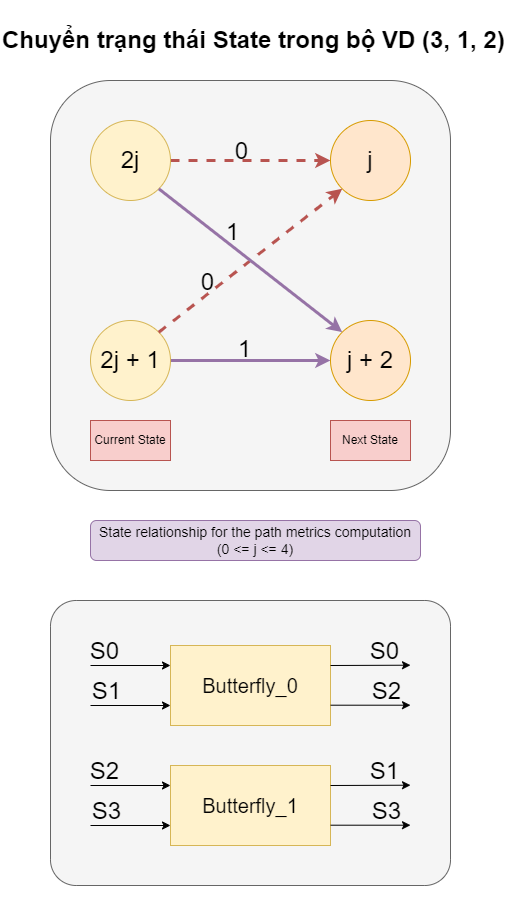
\includegraphics[width=.6\linewidth]{sections/pic/mophongbangSystemVerilog/ACSU_proc_state.png}
	\caption{Cách chuyển trạng thái trong bộ giải mã Viterbi ($3, 1, 2$).}
\end{figure}

\begin{figure}[H]
	\centering
	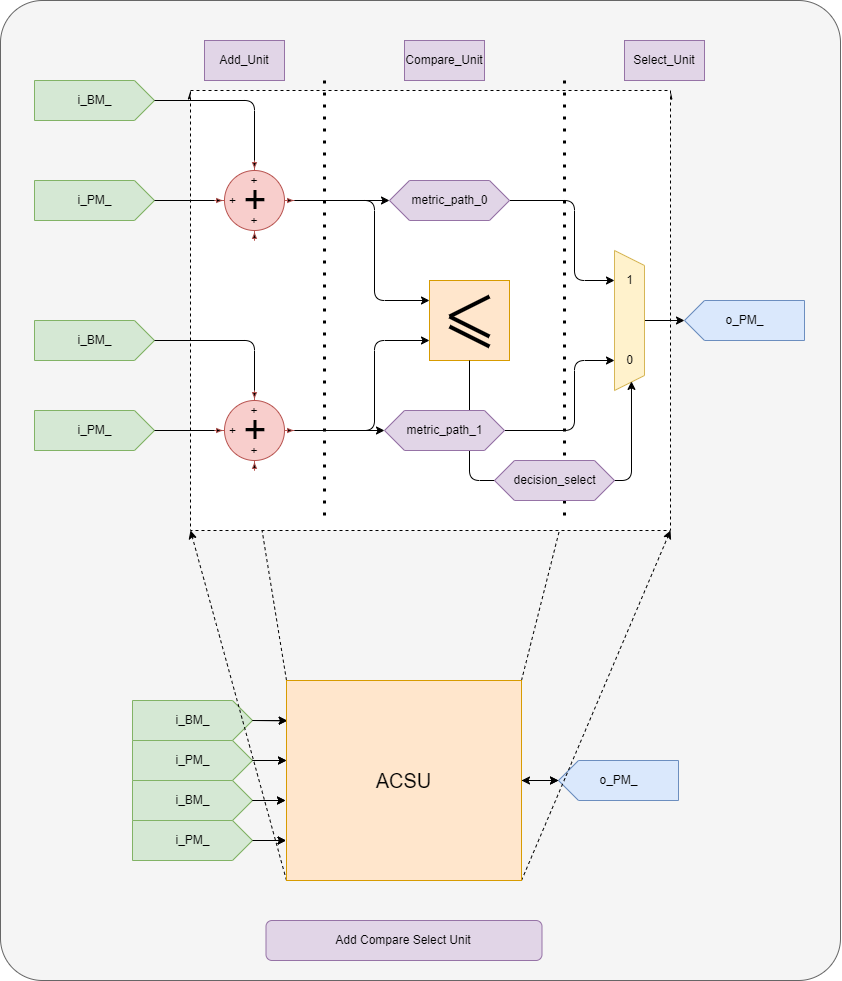
\includegraphics[width=.8\linewidth]{sections/pic/mophongbangSystemVerilog/ACS.png}
	\caption{Bộ Add Compare Select.}
\end{figure}

\begin{figure}[H]
	\centering
	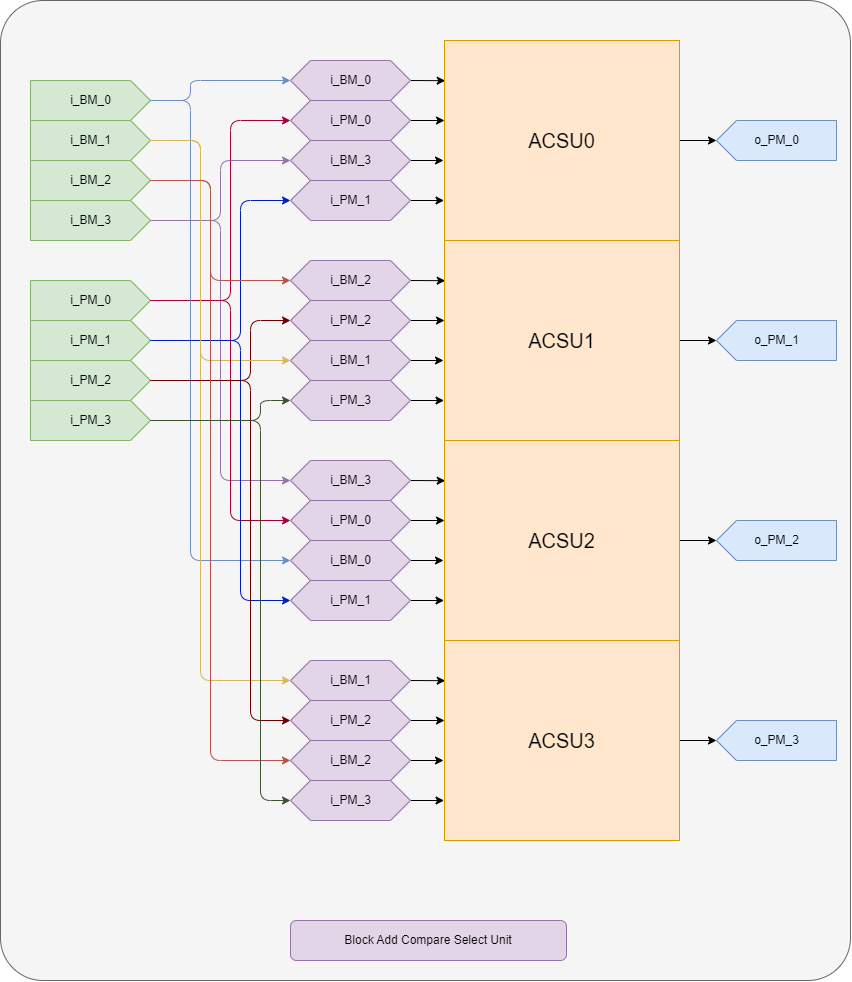
\includegraphics[width=.8\linewidth]{sections/pic/mophongbangSystemVerilog/ACSU.png}
	\caption{Bộ ACSU hoàn chỉnh.}
\end{figure}

\subsubsection{IO for ACSU}

\begin{table}[H]
	\centering
	\begin{tabular}{|>{\centering\arraybackslash}p{3cm}|>{\centering\arraybackslash}p{1cm}|>{\raggedright\arraybackslash}p{9cm}|}
		\hline
		\textbf{Port} & \textbf{Size} & \textbf{Function} \\ \hline
		i\_BM\_0 & 2 & Ngõ vào số liệu nhánh 0 (Branch Metric) \\ \hline
		i\_BM\_1 & 2 & Ngõ vào số liệu nhánh 1 (Branch Metric) \\ \hline
		i\_BM\_2 & 2 & Ngõ vào số liệu nhánh 2 (Branch Metric) \\ \hline
		i\_BM\_3 & 2 & Ngõ vào số liệu nhánh 3 (Branch Metric) \\ \hline
		i\_PM\_0 & 2 & Ngõ vào số liệu đường 0 (Path Metric) \\ \hline
		i\_PM\_1 & 2 & Ngõ vào số liệu đường 1 (Path Metric) \\ \hline
		i\_PM\_2 & 2 & Ngõ vào số liệu đường 2 (Path Metric) \\ \hline
		i\_PM\_3 & 2 & Ngõ vào số liệu đường 3 (Path Metric) \\ \hline
		o\_PM\_0 & 2 & Ngõ ra số liệu đường 0 (Path Metric) \\ \hline
		o\_PM\_1 & 2 & Ngõ ra số liệu đường 1 (Path Metric) \\ \hline
		o\_PM\_2 & 2 & Ngõ ra số liệu đường 2 (Path Metric) \\ \hline
		o\_PM\_3 & 2 & Ngõ ra số liệu đường 3 (Path Metric) \\ \hline
	\end{tabular}
	\caption{Bảng sơ đồ chân của bộ ACSU.}
\end{table}

\subsubsection{Chức năng của ACSU}

Bộ ACSU thực các chức năng chính sau đây:
\begin{itemize}[label=-]
	\item Add: thực hiện chức năng cộng các giá trị Branch Metric ở trạng thái trước đó và giá trị Path Metric hiện tại ở state đó.
	
	Bộ Add Unit trên được thực theo bảng sự thật sau:
	
	\begin{table}[H]
		\centering
		\begin{tabular}{|>{\centering\arraybackslash}p{3cm}|>{\centering\arraybackslash}p{3cm}|>{\centering\arraybackslash}p{3cm}|}
			\hline
			\textbf{i\_BM} & \textbf{i\_PM} & \textbf{o\_PM} \\
			\hline
			00 & 00 & 00 \\
			\hline
			00 & 01 & 01 \\
			\hline
			00 & 10 & 10 \\
			\hline
			00 & 11 & 11 \\
			\hline
			01 & 00 & 01 \\
			\hline
			01 & 01 & 10 \\
			\hline
			01 & 10 & 11 \\
			\hline
			01 & 11 & 11 \\
			\hline
			10 & 00 & 10 \\
			\hline
			10 & 01 & 11 \\
			\hline
			10 & 10 & 11 \\
			\hline
			10 & 11 & 11 \\
			\hline
			11 & 00 & 11 \\
			\hline
			11 & 01 & 11 \\
			\hline
			11 & 10 & 11 \\
			\hline
			11 & 11 & 11 \\
			\hline
		\end{tabular}
		\caption{Bảng sự thật của Add Unit.}
	\end{table}
	
	\begin{lstlisting}[style=StyleResult, language=Result, caption={The Result of testing Add Unit.}]
		Starting Add_unit testbench...
		============================
		TestCase 1 	| Inputs: 00 + 00 	| Output: 00 	| Expected: 00 	| 
		-> PASS
		TestCase 2 	| Inputs: 00 + 01 	| Output: 01 	| Expected: 01 	| 
		-> PASS
		TestCase 3 	| Inputs: 00 + 10 	| Output: 10 	| Expected: 10 	| 
		-> PASS
		TestCase 4 	| Inputs: 00 + 11 	| Output: 11 	| Expected: 11 	| 
		-> PASS
		TestCase 5 	| Inputs: 01 + 00 	| Output: 01 	| Expected: 01 	| 
		-> PASS
		TestCase 6 	| Inputs: 01 + 01 	| Output: 10 	| Expected: 10 	| 
		-> PASS
		TestCase 7 	| Inputs: 01 + 10 	| Output: 11 	| Expected: 11 	| 
		-> PASS
		TestCase 8 	| Inputs: 01 + 11 	| Output: 11 	| Expected: 11 	| 
		-> PASS
		TestCase 9 	| Inputs: 10 + 00 	| Output: 10 	| Expected: 10 	| 
		-> PASS
		TestCase 10 	| Inputs: 10 + 01 	| Output: 11 	| Expected: 11 	| 
		-> PASS
		TestCase 11 	| Inputs: 10 + 10 	| Output: 11 	| Expected: 11 	| 
		-> PASS
		TestCase 12 	| Inputs: 10 + 11 	| Output: 11 	| Expected: 11 	| 
		-> PASS
		TestCase 13 	| Inputs: 11 + 00 	| Output: 11 	| Expected: 11 	| 
		-> PASS
		TestCase 14 	| Inputs: 11 + 01 	| Output: 11 	| Expected: 11 	| 
		-> PASS
		TestCase 15 	| Inputs: 11 + 10 	| Output: 11 	| Expected: 11 	| 
		-> PASS
		TestCase 16 	| Inputs: 11 + 11 	| Output: 11 	| Expected: 11 	| 
		-> PASS
		
		Test Summary:
		=============
		Total tests : 16
		Passed      : 16
		Failed      : 0
		Pass rate   : 100.00%
		- tb_addunit.sv:173: Verilog $finish
	\end{lstlisting}
	
	\item Compare: thực hiện việc so sánh hai giá trị Path Metric hiện tại để kiểm tra xem có giá trị nào hơn để đến bước quyết định.
	
	Bộ Compare Unit trên được thực hiện theo bảng sự thật sau:
	
	\begin{table}[H]
		\centering
		\begin{tabular}{|>{\centering\arraybackslash}p{4cm}|>{\centering\arraybackslash}p{4cm}|>{\centering\arraybackslash}p{4cm}|}
			\hline
			\textbf{i\_metric\_path\_0} & \textbf{i\_metric\_path\_1} & \textbf{o\_compare\_less} \\
			\hline
			00 & 00 & 1 \\ \hline
			00 & 01 & 1 \\ \hline
			00 & 10 & 1 \\ \hline
			00 & 11 & 1 \\ \hline
			01 & 00 & 0 \\ \hline
			01 & 01 & 1 \\ \hline
			01 & 10 & 1 \\ \hline
			01 & 11 & 1 \\ \hline
			10 & 00 & 0 \\ \hline
			10 & 01 & 0 \\ \hline
			10 & 10 & 1 \\ \hline
			10 & 11 & 1 \\ \hline
			11 & 00 & 0 \\ \hline
			11 & 01 & 0 \\ \hline
			11 & 10 & 0 \\ \hline
			11 & 11 & 1 \\ \hline
			\hline
		\end{tabular}
		\caption{Bảng sự thật của bộ Compare Unit.}
	\end{table}
	
	\begin{lstlisting}[style=StyleResult, language=Result, caption={The Result of testing Compare Unit.}]
		Starting Compare_unit testbench...
		=================================
		TestCase 1 	| Inputs: A=00 	 B=00 	| Output: 1 	| Expected: 1 	| 
		-> PASS
		TestCase 2 	| Inputs: A=00 	 B=01 	| Output: 1 	| Expected: 1 	| 
		-> PASS
		TestCase 3 	| Inputs: A=00 	 B=10 	| Output: 1 	| Expected: 1 	| 
		-> PASS
		TestCase 4 	| Inputs: A=00 	 B=11 	| Output: 1 	| Expected: 1 	| 
		-> PASS
		TestCase 5 	| Inputs: A=01 	 B=00 	| Output: 0 	| Expected: 0 	| 
		-> PASS
		TestCase 6 	| Inputs: A=01 	 B=01 	| Output: 1 	| Expected: 1 	| 
		-> PASS
		TestCase 7 	| Inputs: A=01 	 B=10 	| Output: 1 	| Expected: 1 	| 
		-> PASS
		TestCase 8 	| Inputs: A=01 	 B=11 	| Output: 1 	| Expected: 1 	| 
		-> PASS
		TestCase 9 	| Inputs: A=10 	 B=00 	| Output: 0 	| Expected: 0 	| 
		-> PASS
		TestCase 10 	| Inputs: A=10 	 B=01 	| Output: 0 	| Expected: 0 	| 
		-> PASS
		TestCase 11 	| Inputs: A=10 	 B=10 	| Output: 1 	| Expected: 1 	| 
		-> PASS
		TestCase 12 	| Inputs: A=10 	 B=11 	| Output: 1 	| Expected: 1 	| 
		-> PASS
		TestCase 13 	| Inputs: A=11 	 B=00 	| Output: 0 	| Expected: 0 	| 
		-> PASS
		TestCase 14 	| Inputs: A=11 	 B=01 	| Output: 0 	| Expected: 0 	| 
		-> PASS
		TestCase 15 	| Inputs: A=11 	 B=10 	| Output: 0 	| Expected: 0 	| 
		-> PASS
		TestCase 16 	| Inputs: A=11 	 B=11 	| Output: 1 	| Expected: 1 	| 
		-> PASS
		
		Test Summary:
		=============
		Total tests : 16
		Passed      : 16
		Failed      : 0
		Pass rate   : 100.00%
		- tb_compare.sv:151: Verilog $finish
	\end{lstlisting}
	
	\item Select: thực hiện việc quyết định quá trị ngõ ra của giá trị Path Metric với tín hiệu o\_compare\_less từ bộ Compare Unit, việc chọn dữ liệu ngõ ra là thực hiện phép tính nhỏ hơn hoặc bằng ($\leq$).
	
	\begin{table}[H]
		\centering
		\begin{tabular}{|>{\centering\arraybackslash}p{4cm}|>{\centering\arraybackslash}p{4cm}|>{\centering\arraybackslash}p{4cm}|>{\centering\arraybackslash}p{4cm}|}
			\hline
			\textbf{i\_metric\_path\_0} & \textbf{i\_metric\_path\_1} & \textbf{i\_compare\_less} & \textbf{o\_PM}\\
			\hline
			Data\_0 & x & 0 & Data\_0 \\
			\hline
			x & Data\_1 & 1 & Data\_1 \\
			\hline
		\end{tabular}
		\caption{Bảng sự thật của bộ Select Unit.}
	\end{table}
	 
\end{itemize}

Bộ ACSU cần kết hợp thêm bộ PMU (Path Metric Unit) có chức năng lưu giá trị Path Metric của các state tại thời gian trước đó, để có thể giúp.

\begin{lstlisting}[style=StyleResult, language=Result, caption={The Result of testing ACSU.}]
	Time: 110000 	| i_data = 00 	| i_valid = 0 	|
	| i_BM_0: 00 	| i_BM_1: 01 	| i_BM_2: 01 	| i_BM_3: 10 	|
	| i_PM_0: 00 	| i_PM_1: 11 	| i_PM_2: 11 	| i_PM_3: 11 	|
	| o_PM_0: 00 	| o_PM_1: 11 	| o_PM_2: 10 	| o_PM_3: 11 	|
	| t_PM_0: 00 	| t_PM_1: 11 	| t_PM_2: 10 	| t_PM_3: 11 	|
	-> PASS
	=====================================
	Starting ACSU and PMU testbench...
	Time: 130000 	| i_data = 00 	| i_valid = 1 	|
	| i_BM_0: 00 	| i_BM_1: 01 	| i_BM_2: 01 	| i_BM_3: 10 	|
	| i_PM_0: 00 	| i_PM_1: 11 	| i_PM_2: 11 	| i_PM_3: 11 	|
	| o_PM_0: 00 	| o_PM_1: 11 	| o_PM_2: 10 	| o_PM_3: 11 	|
	| t_PM_0: 00 	| t_PM_1: 11 	| t_PM_2: 10 	| t_PM_3: 11 	|
	-> PASS
	=====================================
	=====================================
	Time: 150000 	| i_data = 00 	| i_valid = 1 	|
	| i_BM_0: 00 	| i_BM_1: 01 	| i_BM_2: 01 	| i_BM_3: 10 	|
	| i_PM_0: 00 	| i_PM_1: 11 	| i_PM_2: 10 	| i_PM_3: 11 	|
	| o_PM_0: 00 	| o_PM_1: 11 	| o_PM_2: 10 	| o_PM_3: 11 	|
	| t_PM_0: 00 	| t_PM_1: 11 	| t_PM_2: 10 	| t_PM_3: 11 	|
	-> PASS
	=====================================
	=====================================
	Time: 170000 	| i_data = 01 	| i_valid = 1 	|
	| i_BM_0: 01 	| i_BM_1: 00 	| i_BM_2: 10 	| i_BM_3: 01 	|
	| i_PM_0: 00 	| i_PM_1: 11 	| i_PM_2: 10 	| i_PM_3: 11 	|
	| o_PM_0: 10 	| o_PM_1: 10 	| o_PM_2: 10 	| o_PM_3: 01 	|
	| t_PM_0: 10 	| t_PM_1: 10 	| t_PM_2: 10 	| t_PM_3: 01 	|
	-> PASS
	=====================================
	=====================================
	Time: 190000 	| i_data = 10 	| i_valid = 1 	|
	| i_BM_0: 01 	| i_BM_1: 10 	| i_BM_2: 00 	| i_BM_3: 01 	|
	| i_PM_0: 01 	| i_PM_1: 11 	| i_PM_2: 01 	| i_PM_3: 10 	|
	| o_PM_0: 10 	| o_PM_1: 10 	| o_PM_2: 10 	| o_PM_3: 10 	|
	| t_PM_0: 10 	| t_PM_1: 10 	| t_PM_2: 10 	| t_PM_3: 10 	|
	-> PASS
	=====================================
	=====================================
	Time: 210000 	| i_data = 11 	| i_valid = 1 	|
	| i_BM_0: 10 	| i_BM_1: 01 	| i_BM_2: 01 	| i_BM_3: 00 	|
	| i_PM_0: 10 	| i_PM_1: 01 	| i_PM_2: 10 	| i_PM_3: 10 	|
	| o_PM_0: 11 	| o_PM_1: 11 	| o_PM_2: 01 	| o_PM_3: 11 	|
	| t_PM_0: 11 	| t_PM_1: 11 	| t_PM_2: 01 	| t_PM_3: 11 	|
	-> PASS
	=====================================
	=====================================
	Simulation finished.
	=====================================
	- tb_acsu.sv:359: Verilog $finish
\end{lstlisting}

\subsection{Survivor Path Memory Unit (SPMU)}

\subsubsection{Block Diagram for SPMU}

\begin{figure}[H]
	\centering
	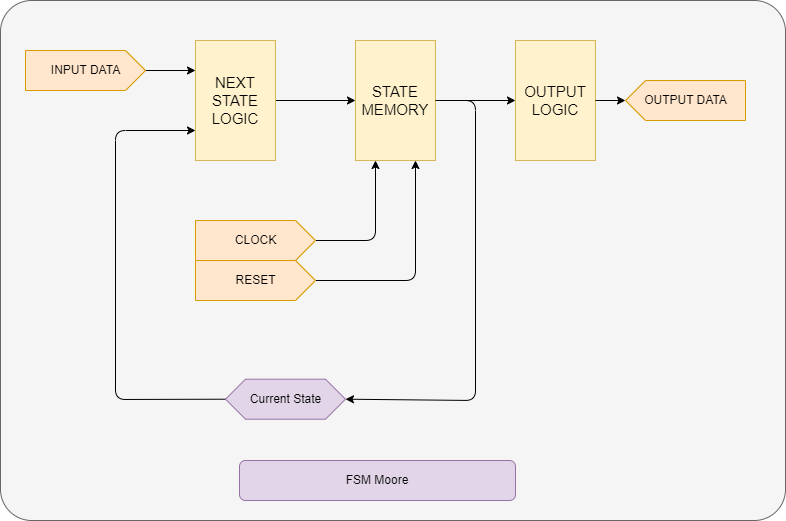
\includegraphics[width=.8\linewidth]{sections/pic/mophongbangSystemVerilog/FSM.png}
	\caption{Máy trạng thái viết ở dạng Moore.}
	\label{f_moore}
\end{figure}

\begin{figure}[H]
	\centering
	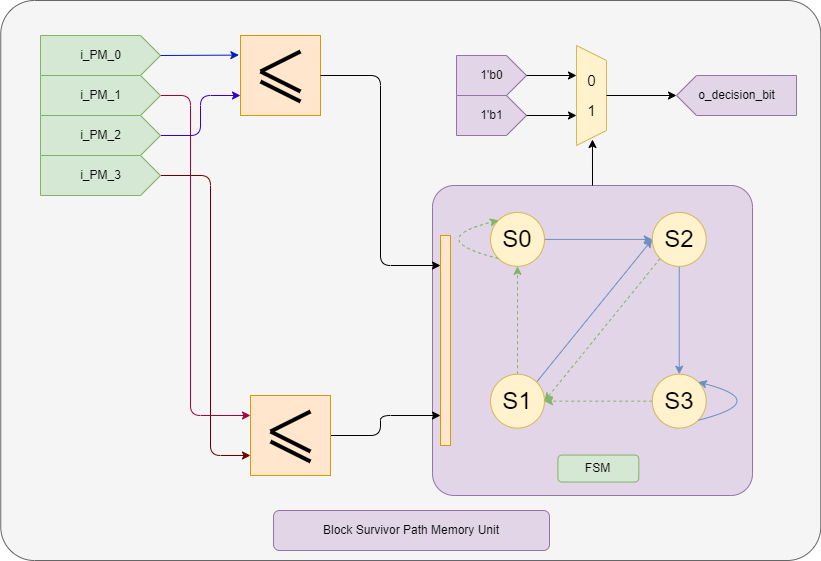
\includegraphics[width=.8\linewidth]{sections/pic/mophongbangSystemVerilog/SPMU.png}
	\caption{Bộ SPMU.}
\end{figure}

\subsubsection{IO for SPMU}

\begin{table}[H]
	\centering
	\begin{tabular}{|>{\centering\arraybackslash}p{3cm}|>{\centering\arraybackslash}p{1cm}|>{\raggedright\arraybackslash}p{9cm}|}
		\hline
		\textbf{Port} & \textbf{Size} & \textbf{Function} \\
		\hline
		i\_clk & 1 & Xung clock hệ thống \\
		\hline
		i\_rst\_n & 1 & Tín hiệu reset tích cực mức thấp \\
		\hline
		i\_valid & 1 & Tín hiệu valid cho dữ liệu vào \\
		\hline
		i\_PM\_0 & 2 & Giá trị Path Metric 0 đầu vào \\
		\hline
		i\_PM\_1 & 2 & Giá trị Path Metric 1 đầu vào \\
		\hline
		i\_PM\_2 & 2 & Giá trị Path Metric 2 đầu vào \\
		\hline
		i\_PM\_3 & 2 & Giá trị Path Metric 3 đầu vào \\
		\hline
		o\_decision & 1 & Quyết định đường đi tối ưu (0-3) \\
		\hline
		o\_valid & 1 & Tín hiệu valid cho dữ liệu ra \\
		\hline
	\end{tabular}
	\caption{Bảng sơ đồ chân của bộ SPMU (Survivor Path Memory Unit).}
	\label{tab:spmu_ports}
\end{table}

\subsubsection{Chức năng của bộ SMPU}

Bộ SPMU có nhiệm vụ quyết định bit ngõ ra dữ vào bit đầu vào. Có thể coi bộ SPMU là một nhân xử lý chính trong bộ VD giúp quyết định bit ngõ ra là gì. Bộ SPMU được viết dự vào máy trạng thái với các trạng chính trong trellis thể hiện ở hình \ref{f_trellis_unit_conv_encoder}. Như vậy, ta có thể thấy được ngõ ra được quyết định bởi trạng thái hiện tại và trạng thái tiếp chứ không phụ thuộc vào điều kiện ngõ vào, nên ta sử dụng mô hình moore như hình \ref{f_moore}, giúp cho dữ liệu ngõ được ổn định và chính xác hơn.

Sơ đồ quyết định bit ngõ ra dữ vào trạng thái hiện và trạng ngõ ra như sau:

\begin{figure}[H]
	\centering
	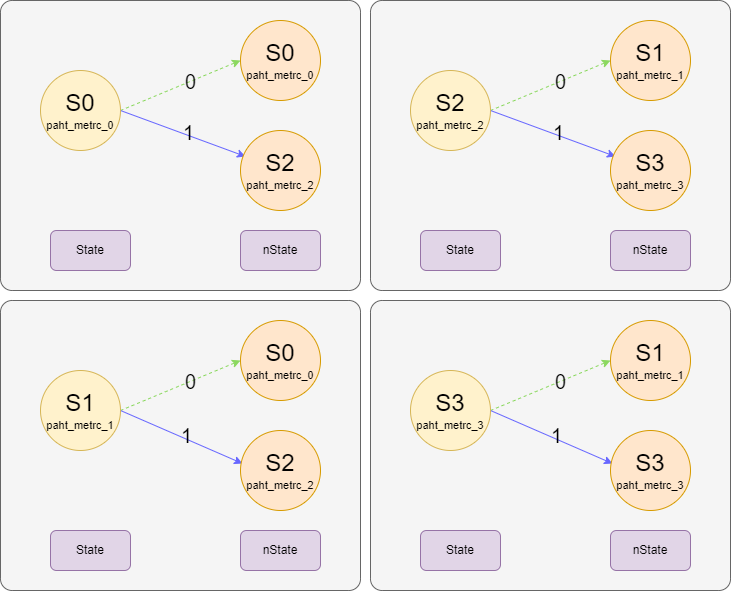
\includegraphics[width=.8\linewidth]{sections/pic/mophongbangSystemVerilog/spmu_trans.png}
	\caption{Sơ đồ quyết định bit ngõ ra của bộ SPMU.}
\end{figure}

%\begin{lstlisting}[style=StyleResult, language=Result]
%	Time =                 5000 	| i_rst_n = 1 	| o_decision = 0 	| o_valid = 0 	|
%	PM_0 = 0 	| PM_1 = 0 	| PM_2 = 0 	| PM_3 = 0 	| 
%	=========================================
%	case 1: S0 -> S0
%	Time = 15000 	| i_rst_n = 1 	| o_decision = 0 	| o_valid = 1 	|
%	PM_0 = 0 	| PM_1 = 1 	| PM_2 = 2 	| PM_3 = 3 	| 
%	=========================================
%	case 2: S0 -> S2
%	Time = 25000 	| i_rst_n = 1 	| o_decision = 0 	| o_valid = 1 	|
%	PM_0 = 3 	| PM_1 = 2 	| PM_2 = 1 	| PM_3 = 0 	| 
%	=========================================
%	case 3: S2 -> S1
%	Time = 35000 	| i_rst_n = 1 	| o_decision = 1 	| o_valid = 1 	|
%	PM_0 = 2 	| PM_1 = 0 	| PM_2 = 0 	| PM_3 = 1 	| 
%	=========================================
%	case 4: S1 -> S2
%	Time = 45000 	| i_rst_n = 1 	| o_decision = 1 	| o_valid = 1 	|
%	PM_0 = 3 	| PM_1 = 0 	| PM_2 = 1 	| PM_3 = 2 	| 
%	=========================================
%	case 5: S2 -> S3
%	Time = 55000 	| i_rst_n = 1 	| o_decision = 0 	| o_valid = 1 	|
%	PM_0 = 1 	| PM_1 = 2 	| PM_2 = 3 	| PM_3 = 0 	| 
%	=========================================
%	case 6: S3 -> S3
%	Time = 65000 	| i_rst_n = 1 	| o_decision = 1 	| o_valid = 1 	|
%	PM_0 = 3 	| PM_1 = 2 	| PM_2 = 1 	| PM_3 = 0 	| 
%	=========================================
%	Testbench completed successfully
%	==================================
%	- tb_spmu.sv:113: Verilog $finish
%\end{lstlisting}
\begin{lstlisting}[style=StyleResult, language=Result, caption={The result of testing SPMU}]
	Time = 	5000 | i_rst_n = 1 	| i_valid = 0 	| o_decision = 0 	 |
	PM_0 = 00  	 | PM_1 = 00 	| PM_2 = 00 	| PM_3 = 00 	     |
	=========================================
	TestCase 1: S0 -> S0
	Time =  16000 | i_rst_n = 1 	| i_valid = 1 	| o_decision = 0 |
	PM_0 = 00 	  | PM_1 = 01 	| PM_2 = 10 	| PM_3 = 11 	     |
	-> PASS
	=========================================
	TestCase 2: S0 -> S2
	Time = 26000 | i_rst_n = 1 	| i_valid = 1 	| o_decision = 1 	 |
	PM_0 = 11 	 | PM_1 = 10 	| PM_2 = 01 	| PM_3 = 00 	     |
	-> PASS
	=========================================
	TestCase 3: S2 -> S1
	Time = 36000 | i_rst_n = 1 	| i_valid = 1 	| o_decision = 0     |
	PM_0 = 10 	 | PM_1 = 00 	| PM_2 = 00 	| PM_3 = 01 	     |
	-> PASS
	=========================================
	TestCase 4: S1 -> S2
	Time = 46000 | i_rst_n = 1 	| i_valid = 1 	| o_decision = 1 	 |
	PM_0 = 11 	 | PM_1 = 00 	| PM_2 = 01 	| PM_3 = 10 	     |
	-> PASS
	=========================================
	TestCase 5: S2 -> S3
	Time = 56000 | i_rst_n = 1 	| i_valid = 1 	| o_decision = 1 	 |
	PM_0 = 01 	 | PM_1 = 10 	| PM_2 = 11 	| PM_3 = 00 	     |
	-> PASS
	=========================================
	TestCase 6: S3 -> S3
	Time = 66000 | i_rst_n = 1 	| i_valid = 1 	| o_decision = 1 	 |
	PM_0 = 11  	 | PM_1 = 10 	| PM_2 = 01 	| PM_3 = 00 	     |
	-> PASS
	=========================================
	TestCase 7: S3 -> S1
	Time = 76000 | i_rst_n = 1 	| i_valid = 1 	| o_decision = 0 	 |
	PM_0 = 11 	 | PM_1 = 00 	| PM_2 = 01 	| PM_3 = 10 	     |
	-> PASS
	=========================================
	TestCase 8: S1 -> S0
	Time = 86000 | i_rst_n = 1 	| i_valid = 1 	| o_decision = 0 	|
	PM_0 = 00 	 | PM_1 = 01 	| PM_2 = 01 	| PM_3 = 10 	    |
	-> PASS
	=========================================
	Testbench completed successfully
	==================================
	- tb_spmu.sv:168: Verilog $finish
\end{lstlisting}

\subsection{Viterbi Decoder Block}

\subsubsection{Block Diagram for Viterbi Decoder Block}

\begin{figure}[H]
	\centering
	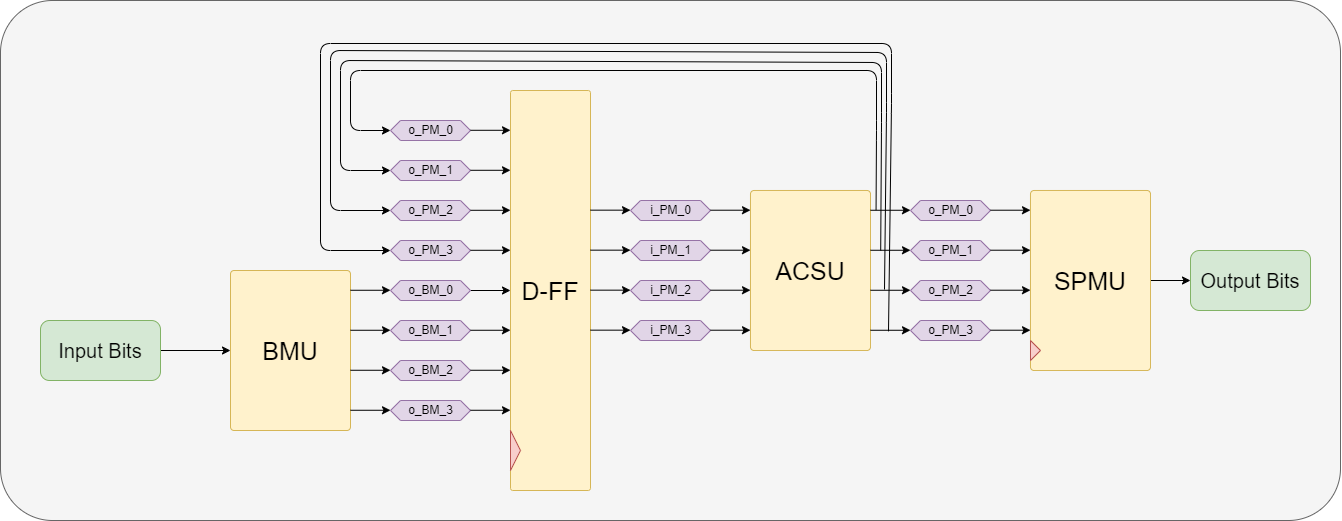
\includegraphics[width=.7\linewidth]{sections/pic/mophongbangSystemVerilog/viterbi_decoder.png}
	\caption{Bộ Viterbi Decoder.}
\end{figure}

\subsubsection{IO for Viterbi Decoder Block}

\begin{table}[H]
	\centering
	\begin{tabular}{|>{\centering\arraybackslash}p{3cm}|>{\centering\arraybackslash}p{1cm}|>{\raggedright\arraybackslash}p{9cm}|}
		\hline
		\textbf{Port} & \textbf{Size} & \textbf{Function} \\
		\hline
		i\_clk & 1 & Xung nhịp hệ thống \\
		\hline
		i\_rst\_n & 1 & Tín hiệu reset tích cực mức thấp (Active-low reset) \\
		\hline
		i\_valid & 1 & Tín hiệu báo dữ liệu vào hợp lệ \\
		\hline
		i\_data & 2 & Dữ liệu đầu vào cần giải mã \\
		\hline
		o\_decision & 1 & Bit dữ liệu đã được giải mã \\
		\hline
		o\_valid & 1 & Tín hiệu báo dữ liệu ra hợp lệ \\
		\hline
	\end{tabular}
	\caption{Bảng sơ đồ chân của bộ Viterbi Decoder Block.}
\end{table}

%\begin{lstlisting}[style=StyleResult, language=Result]
%	Time= 115000 | i_rst_n=1 | i_start=1 | i_data=1101010001010011 |
%	| o_data=11011010 | o_valid=1| 
%	-> PASS - BER_in=1.000000, BER_out=0.000000
%	Time= 225000 | i_rst_n=1 | i_start=1 | i_data=1110001000100011 |
%	| o_data=10101010 | o_valid=1 |
%	-> PASS - BER_in=1.000000, BER_out=0.000000
%	Time= 335000 | i_rst_n=1 | i_start=1 | i_data=0000000000000111 | 
%	| o_data=00000001 | o_valid=1 | 
%	-> PASS - BER_in=1.000000, BER_out=0.000000
%	Time= 445000 | i_rst_n=1 | i_start=1 | i_data=0000110101111101 |
%	| o_data=00110011 | o_valid=1 |
%	-> PASS - BER_in=0.000000, BER_out=0.000000
%	=========================================
%	Testbench completed successfully
%	=========================================
%	- tb_viterbi.sv:105: Verilog $finish
%\end{lstlisting}

\begin{lstlisting}[style=StyleResult, language=Result]
	Time: 0, o_decision: 0, o_valid: 0
	TestCase 1:
	Data input: 10101010
	Data conv : 1110001000100010
	Time: 50000, o_decision: 1, o_valid: 1
	Time: 51000  | i_valid = 1 	| i_data: 11 | o_decision = 1 | o_valid = 1 |
	Time: 71000  | i_valid = 1 	| i_data: 10 | o_decision = 0 | o_valid = 1 |
	Time: 91000  | i_valid = 1 	| i_data: 00 | o_decision = 1 | o_valid = 1 |
	Time: 111000 | i_valid = 1 	| i_data: 10 | o_decision = 0 | o_valid = 1 |
	Time: 131000 | i_valid = 1 	| i_data: 00 | o_decision = 1 | o_valid = 1 |
	Time: 151000 | i_valid = 1 	| i_data: 10 | o_decision = 0 | o_valid = 1 |
	Time: 171000 | i_valid = 1 	| i_data: 00 | o_decision = 1 | o_valid = 1 |
	Time: 191000 | i_valid = 1 	| i_data: 10 | o_decision = 0 | o_valid = 1 |
	Time: 210000 | i_valid = 1 	| i_data: 10 | o_decision = 0 | o_valid = 1 |
	==========================================================
	Time: 210000, o_decision: 0, o_valid: 0
	TestCase 2:
	Data input: 00101001
	Data conv : 0000111000101111
	Time: 250000, o_decision: 0, o_valid: 1
	Time: 271000 | i_valid = 1 	| i_data: 00 | o_decision = 0 | o_valid = 1 |
	Time: 291000 | i_valid = 1 	| i_data: 00 | o_decision = 0 | o_valid = 1 |
	Time: 311000 | i_valid = 1 	| i_data: 11 | o_decision = 1 | o_valid = 1 |
	Time: 331000 | i_valid = 1 	| i_data: 10 | o_decision = 0 | o_valid = 1 |
	Time: 351000 | i_valid = 1 	| i_data: 00 | o_decision = 1 | o_valid = 1 |
	Time: 371000 | i_valid = 1 	| i_data: 10 | o_decision = 0 | o_valid = 1 |
	Time: 391000 | i_valid = 1 	| i_data: 11 | o_decision = 0 | o_valid = 1 |
	Time: 411000 | i_valid = 1 	| i_data: 11 | o_decision = 1 | o_valid = 1 |
	Time: 430000 | i_valid = 1 	| i_data: 11 | o_decision = 1 | o_valid = 1 |
	==========================================================
	- tb_Viterbi_decoding.sv:119: Verilog $finish
\end{lstlisting}

